% =================== CG properties =================== %
\subsection{Objective}
\begin{frame}[t]{Objective}
\begin{itemize}
    \item Evaluate the impact of \textbf{graph symmetry} on the \textbf{performance} and \textbf{robustness} of parallel computer systems.
    \item Aspects to evaluated:
    \begin{itemize}
        \item Connectivity
        \item Fault-tolerance
        \item Load balancing
    \end{itemize}
    \item Evaluated topologies:
    \begin{itemize}
        \item 3 symmetric Cayley Graphs (CG)
        \item 2 non-symmetric CG
        \item 3 Data Center Networks (DCN)
    \end{itemize}
\end{itemize}
\end{frame}
% =================== CG =================== %
\subsection{Cayley Graphs}
\begin{frame}[t]{Cayley Graphs}
\begin{itemize}
    \item A CG is a geometric representation of an algebraic group.
    \item CGs have regular degree ($\Delta$) and grow increasing their degree.
\end{itemize}
\scriptsize
\begin{table}[]
\centering{
\begin{tabular}[center]{c c c}
\includegraphics{images/tikz/square.tikz}
&\includegraphics{images/tikz/cube.tikz}
&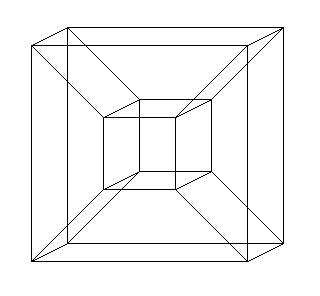
\includegraphics[width=0.245\textwidth]{images/cube4}
\\
\textbf{$\Delta=2$}&\textbf{$\Delta=3$}&\textbf{$\Delta=4$}\\
\end{tabular}
\caption{Family of Hypercube graphs}
}
\end{table}
\end{frame}
% =================== CG properties =================== %
%\begin{frame}[t]{Cayley Graphs: Properties}
%\begin{itemize}
%    \item Recursive graphs.
%    \item Node-transitive.
%    \item Some CGs have constant degree or constant diameter.
%\end{itemize}
%\scriptsize
%\begin{table}[]
%\centering{
%\begin{tabular}[center]{c c c}
%\includegraphics{images/tikz/square.tikz}
%&\includegraphics{images/tikz/cube.tikz}
%&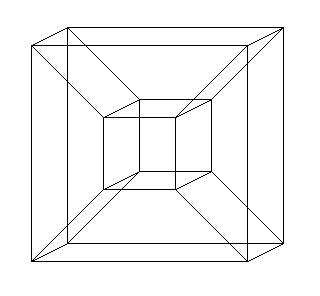
\includegraphics[width=0.245\textwidth]{images/cube4}
%\\
%\textbf{$\Delta=2$}&\textbf{$\Delta=3$}&\textbf{$\Delta=4$}\\
%\end{tabular}
%\caption{Family of Hypercube graphs}
%}
%\end{table}
%\end{frame}
%========================================= %
\begin{frame}{Cayley graphs as Model of Interconnection Networks}
\begin{itemize}
\item Processor Interconnection Networks (PIN) [1-2].
\item Data Center Networks (DCN) [3-4].
\end{itemize}
\center{
    \begin{tabular}{c c c}
        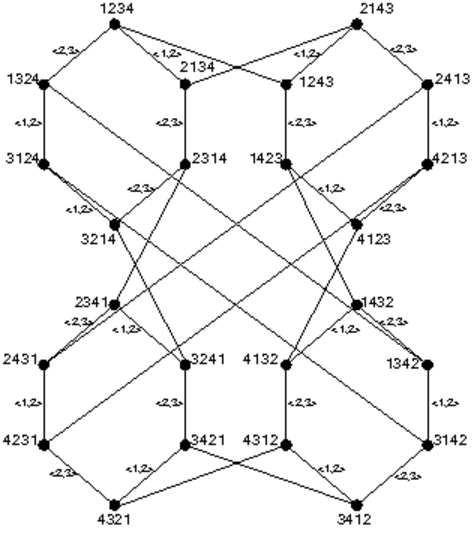
\includegraphics[width=0.25\textwidth]{images/nets/bubble_sort.pdf}
        %& 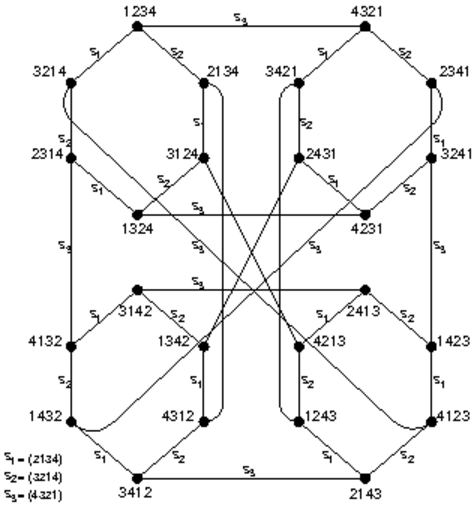
\includegraphics[width=0.3\textwidth]{images/nets/pancake.pdf}
        &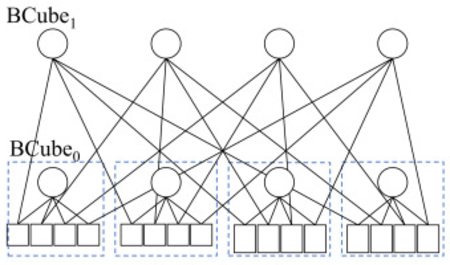
\includegraphics[width=0.5\textwidth]{images/nets/bcube.pdf}\\
        \textbf{\footnotesize Star}
        %& \textbf{\footnotesize Pancake}
        & \textbf{\footnotesize Bcube}\\
    \end{tabular}    }
\flushleft{\tiny
\begin{enumerate}[{[1]}]
	\item M. Heydemann, "Cayley graphs and interconnection networks," on NATO ASI Series: Mathematical and Physical Sciences, vol 497. Springer, 1997. 
    \item T. Stephen et. all, "Processor interconnection networks from Cayley graphs," in Discrete Applied Mathematics, vol. 40, 1992. 
    \item Ch. Guo et. all, "BCube: a high performance, server-centric network architecture for modular data centers,"  in Proc. of the ACM-SIGCOMM, 2009. 
    \item J. Kim et. all, "Flattened butterfly: a cost-efficient topology for high-radix networks,"  in Proc. of the ISCA, 2007. 
    %\item B. Andruset. all, "SDN data center performance evaluation of torus and hypercube interconnecting schemes,"  in Proc. of the RTUWO, 2015.
\end{enumerate}}
\end{frame} 
%========================================= %
%\begin{frame}{Cayley graphs as Models of Interconnection Networks (2/2)}
%\begin{itemize}
%\item Data Center Networks (DCN)\end{itemize}
%\center{
%    \begin{tabular}{c c c}
%        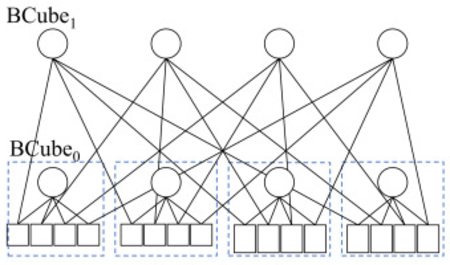
\includegraphics[width=0.28\textwidth]{images/nets/bcube.pdf}& 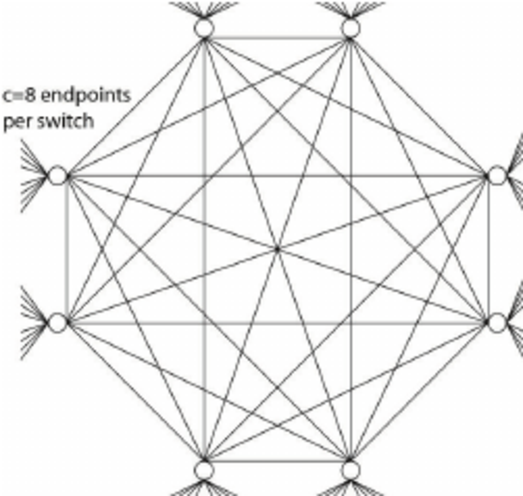
\includegraphics[width=0.21\textwidth]{images/nets/butterfly.pdf}&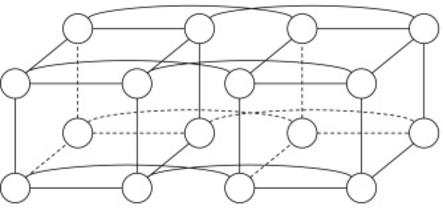
\includegraphics[width=0.28\textwidth]{images/nets/hypercube.pdf}\\
%        \textbf{\footnotesize BCube [3]}& \textbf{\footnotesize Flattened Butterfly [4]}& \textbf{\footnotesize Hypercube [5]}\\
%    \end{tabular}  }
%\flushleft{\tiny
%\begin{enumerate}[{[1]}]
%    \setcounter{enumi}{2}
%	\item Ch. Guo et. all, "BCube: a high performance, server-centric network architecture for modular data centers,"  in Proc. of the ACM-SIGCOMM, 2009. 
%    \item J. Kim et. all, "Flattened butterfly: a cost-efficient topology for high-radix networks,"  in Proc. of the ISCA, 2007. 
%    \item B. Andruset. all, "SDN data center performance evaluation of torus and hypercube interconnecting schemes,"  in Proc. of the RTUWO, 2015.
%\end{enumerate}}
%\end{frame}